\documentclass[10pt]{beamer}

\usepackage{graphicx}

\usetheme{metropolis}
\usepackage{appendixnumberbeamer}

\usepackage{booktabs}
\usepackage[scale=2]{ccicons}

\usepackage{pgfplots}
\usepgfplotslibrary{dateplot}

\usepackage{xspace}
\newcommand{\themename}{\textbf{\textsc{metropolis}}\xspace}

\title{A Future Perspective:}
\subtitle{Exploiting Decentralized Web for Pragmatic Interoperability}
\date{November 21, 2018}
\author{\textbf{Dr. Bambang Purnomosidi}}
\institute{Informatics Engineering Department\\STMIK AKAKOM}
\titlegraphic{\hfill
\includegraphics[height=1.5cm]{isriti-logo.png}}

\begin{document}

\maketitle

\begin{frame}[allowframebreaks]{Table of contents}
  \setbeamertemplate{section in toc}[sections numbered]
  \setbeamertemplate{subsection in toc}{\leavevmode\leftskip=3.2em\rlap{\hskip-2em\inserttocsectionnumber.\inserttocsubsectionnumber}\inserttocsubsection\par}
  \tableofcontents
  %\tableofcontents[hideallsubsections]
\end{frame}

\section{Introduction}

  \subsection{Overview}

    \begin{frame}[fragile]{Overview}

  The World Wide Web (or the Web) is currently consists of many technologies, ecosystems, and virtual resources. Until now, most interactions on the Web happen between client and server. This situation leads to centralized Web where organzations and / or people put their services on the Web for mass consumption by clients. While this situation is normal, centralized Web gives negative impacts for society. Centralized Web gives power to service provider. By building Web to a more decentralized system, we may put power into clients / peers, therefore opening possibilities for customization and interoperability. The decentralized Web empowers creation and encourages participation, hence enable people to create, personalize, and share resources. This talk is a glimpse into pragmatic interoperability by exploiting possibilities from decentralized Web and how we might put pragmatic interoperability into our resources on the (decentralized) Web for the benefit of society as a whole.

    \end{frame}

  \subsection{Web and Decentralized Web}

    %\begin{frame}[allowframebreaks]{Web and Decentralized Web}
    \begin{frame}[fragile]{Web and Decentralized Web}

      \begin{itemize}
        \item Web is a platform which consists of front end resources (HTML, CSS, pictures, videos, JavaScript), rendered by Web browser. Those resources might be static or produced by backend processing. 
        \item Current Web is distributed but mostly have centralized points of control.
        \item This situation puts people in weak position compared with government, private companies or any other big organization. Sensor and surveillance from government are possible. Private companies may use people's data without their consent.
        \item Many layers for people who want to create services and participate.
      \end{itemize}

    \end{frame}

    \begin{frame}[fragile]{Let's Make the Web More Decentralized!}

      To reach a mainstream status, there is no easy for decentralied Web. At the minimum, there has to be a smooth transition from current Web into a more decentralied system. How can we achieve that? At least there are two components which need to be exist:

      \begin{itemize}
        \item A protocol to replace HTTP so that people may put their resources online.
        \item A browser for that protocol.
      \end{itemize}

      Enter \textbf{Dat} protocol and \textbf{Beaker Browser}. \textbf{Solid} (https://solid.inrupt.com/) also maybe of interest.

    \end{frame}

  \subsection{Interoperability}

    \begin{frame}[fragile]{Interoperability}

      \textbf{Interoperability} is the ability of different computer system to exchange and make use data / information from each other. From linguistics point of view, it is the same as two different person are able to understand each other when they both send/receive messages. There are three components of interoperability:
      \begin{itemize}
        \item Syntactic interoperability: both nodes should agree on data serialization format
        \item Semantic interoperability: both nodes can read the data serialization and know the "meaning" of that data (in context independent setting).
        \item Pragmatic interoperablity: both nodes can understand context and intention of message from data / information that they both send/receive.
      \end{itemize}

    \end{frame}

\section{Interoperability on the Web}

  \subsection{Interoperability and the Web}

    \begin{frame}[fragile]{Interoperability and the Web}

      When we talk about interoperability on the Web, we talk about machine to machine communication, not between human. This makes it possible to consume data and doing any automatic intelligent things with data.

    \end{frame}

  \subsection{Syntactic Interoperability on the Web}

    \begin{frame}[fragile]{Syntactic Interoperability on the Web}

      Syntactic interoperability becomes a very basic interoperability on the Web. To achieve syntactic interoperability, data serialization format should be understood by each node. This has now becomes common: XML, JSON, BSON, MessagePack, Protocol Buffer, etc.

    \end{frame}

  \subsection{Semantic Interoperability on the Web}

    \begin{frame}[fragile]{Semantic Interoperability on the Web}
      Semantic interoperability is achieved when both side can exchange and understand the "meaning" of data in a context independent setting. This has become a big concern since around 2001 when people realize that the Web is more for human then for machine. Since that time, many efforts have been done on putting ontology on the Web: DAML/OIL, OWL, OWL2, RDF, Linked Data, etc. 
    \end{frame}

  \subsection{Interoperability and Decentralized Web}

    \begin{frame}[fragile]{Interoperability and Decentralized Web}

      As the Web now becomes centralized, we rely on large-scale server-side infrastructures to perform intense reasoning, data mining, query execution, etc. By using decentralized (for example, using Dat protocol), we may put our resources online in a common data serialization format (syntactic interoperability) with ontology attached or linked data (semantic interoperability) if needed. These are all now can be under control of people and communities.

    \end{frame}

\section{Pragmatic Interoperability and Decentralized Web}

  \subsection{Requirements for Pragmatic Interoperability}

    \begin{frame}[fragile]{Requirements for Pragmatic Interoperability}
      \begin{itemize}
        \item Pragmatics: study how context contributes to meaning. The ability to understand pragmatic in conversation is called \textbf{pragmatic competence}.
        \item Client and service provider is said to be capable of doing contextual and pragmatic interactions if both side can accommodate context in conversation and both understand intention of each side within the same context.
        \item From here, there are 2 important components: \textbf{context} and \textbf{intention}
      \end{itemize}
    \end{frame}

    \begin{frame}[fragile]{Context}
      \begin{itemize}
        \item Context is any relevan data for service provisioning
        \item Since client and service provider has their own context, interoperability becomes inherent problem
        \item One may put context as global file inside his / her resources, and also put context for every resource inside a folder. Context should be described as \textbf{graph abstract data type} and this has to be defined as community consensus. 
        \item Use JSON-LD might be used as a candidate to solve interoperability problem
      \end{itemize}
    \end{frame}

    \begin{frame}[fragile]{Intention}

In a message, \textit{intention} is known as \textit{illocutionary force}, while content of intention is known as \textit{propositional contents}. Communication is developed based on model~\ref{eqn:spcillo}.

\begin{equation}\label{eqn:spcillo}
  \boxed{f(p)}
\end{equation}

where:

\begin{description}
  \item[$f$] represent \textit{illocutionary force}
  \item[$p$] represent \textit{propositional contents}
\end{description}

    \end{frame}

    \begin{frame}[fragile]{Illocutionary Force}

\begin{itemize}
  \item \textit{Representatives}: states that something is true. This rule consists of \textit{assertive} (``ASSERT'' keyword) and \textit{informative} (``INFORM'' keyword).
  \item \textit{Directives}: cause the hearer to take a particular action, consists only ``REQUEST'' keyword.
  \item \textit{Commissives}: making a commitment, such as a promise or threat, by illocutionary means (such as ``I will buy if you give me 30 percent discounts'').
  \item  \textit{Expressives}: express the speaker's attitudes and emotions towards the proposition, e.g. congratulations, excuses and thanks ( ``APOLOGIZE'', ``THANK'', and ``COMPLAIN'' keywords).
  \item \textit{Declaratives}: change the reality in accord with the proposition of the declaration, e.g. pronouncing someone guilty or pronouncing someone husband and wife (``DECLARE'' keyword).
\end{itemize}

    \end{frame}

  \subsection{Architecture of Decentralized Web Components for Pragmatic Interoperability}

    \begin{frame}[fragile]{Architecture of Decentralized Web Components for Pragmatic Interoperability}

      \begin{figure}[h]
      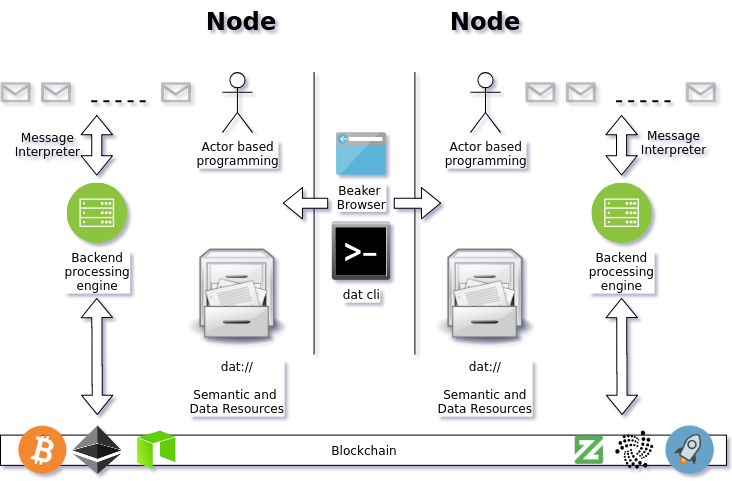
\includegraphics[scale=0.4]{decweb-pragmatic-int}
      \end{figure}

    \end{frame}

  \subsection{Impact for Society}

    \begin{frame}[fragile]{Impact for Society}
      \begin{itemize}
        \item More powerful clients, providing balance of power between any entities and people.
        \item Difficult for censorship and surveillance
        \item Robust: there is no single node which can take the whole network down.
        \item Eliminate middleman, hence reduce costs and complexities
        \item Decentralized data analytics.
        \item Total control of data in people
      \end{itemize}
    \end{frame}

  \subsection{Research Challenges}

    \begin{frame}[fragile]{Research Challenges}
      \begin{itemize}
        \item (Global) Identity and an official identity mapping with offline ID
        \item Context taxonomy and management
        \item Actor-based programming tools
        \item Message interpreter
        \item Semantic infrastructure
        \item InterLedger protocol
      \end{itemize}
    \end{frame}

\end{document}
